\section{Results}
\label{sec:results}
The results follow the endpoints: first the accuracy curve with its onset and slope, then the classes on which the damage lands, the position of the native allocation, and finally probability quality before and after temperature scaling. The balanced arm reaches 72.06 percent balanced accuracy (70.68 to 73.31). Twenty patients with eight patches each reached 71.89 percent in \citet{queisler2026centreError}; the fourfold patch depth of this design therefore changes the balanced reference by less than a fifth of a point, as expected on TCGA-UT, where patch depth hardly matters.

\subsection{Accuracy curve}
\label{sec:curve-results}
Balanced accuracy falls monotonically with the imbalance ratio, slowly at first and then faster (Table~\ref{tab:curve}, Figure~\ref{fig:curve}). Already $\rho=2$ costs a resolved 0.11 points (0.01 to 0.21), but the damage stays below half a point up to $\rho=5$ and reaches 0.57 points (0.30 to 0.84) at $\rho=10$. At $\rho=20$ it is 1.01 points (0.67 to 1.36), so the onset of the grid is $\rho=20$, although the lower bound of its interval still lies below one point. At $\rho=50$ the damage is 1.85 points (1.47 to 2.24), and at $\rho=100$ it is 2.91 points (2.48 to 3.34), with the whole interval above the threshold. The three splits agree closely: the damage at $\rho=100$ is 2.96, 2.90, and 2.88 points.

\begin{table}[htbp]
\centering
\small
\setlength{\tabcolsep}{4pt}
\renewcommand{\arraystretch}{1.15}
\begin{tabular}{@{}lrrrrrrr@{}}
\toprule
 & & & \multicolumn{2}{c}{Macro NLL (nats)} & \multicolumn{2}{c}{ECE (points)} & \\
\cmidrule(lr){4-5}\cmidrule(lr){6-7}
Arm & BA (\%) & Damage $\Delta$ & raw & scaled & raw & scaled & Temperature \\
\midrule
r1 & 72.06 & --- & 0.943 & 0.921 & 5.50 & 1.52 & 0.84 \\
r2 & 71.94 & 0.11 [0.01, 0.21] & 0.950 & 0.928 & 5.52 & 1.56 & 0.93 \\
r5 & 71.68 & 0.37 [0.14, 0.60] & 0.967 & 0.944 & 6.06 & 1.56 & 1.14 \\
r10 & 71.48 & 0.57 [0.30, 0.84] & 0.983 & 0.952 & 6.54 & 1.65 & 1.20 \\
r20 & 71.05 & \textbf{1.01} [0.67, 1.36] & 1.091 & 0.974 & 10.45 & 1.74 & 1.44 \\
r50 & 70.21 & \textbf{1.85} [1.47, 2.24] & 1.178 & 1.008 & 13.43 & 1.96 & 1.59 \\
r100 & 69.14 & \textbf{2.91} [2.48, 3.34] & 1.605 & 1.046 & 17.80 & 2.08 & 2.35 \\
\addlinespace
N ($\rho=18.1$) & 70.88 & \textbf{1.18} [0.85, 1.48] & 1.080 & 0.976 & 8.86 & 1.39 & 1.40 \\
\bottomrule
\end{tabular}
\caption{Accuracy degrades slowly with prevalence, raw probability quality much faster, and temperature scaling removes most of the probability-quality loss. Balanced accuracy (BA) is test patient-macro balanced accuracy; the damage is $\mathrm{BA}(1)-\mathrm{BA}(\rho)$ in percentage points with paired 95\% bootstrap intervals, in bold where it meets the one-point criterion. NLL and ECE are shown without (raw) and with (scaled) the validation temperature; the temperature column is the mean fitted temperature over 30 fits, where values above one soften overconfident predictions. The 95\% intervals of the absolute BA levels are about 2.6 points wide and are shared by all arms.}
\label{tab:curve}
\end{table}

\noindent The loss per doubling of $\rho$ is 0.41 points (0.35 to 0.48) over the whole grid, but the curve is not linear in $\log\rho$. Up to $\rho=10$ it loses 0.18 points per doubling (0.09 to 0.26), from $\rho=10$ to $\rho=100$ it loses 0.70 points (0.63 to 0.76), and the two intervals do not overlap. The damage thus accelerates as the tail classes approach one or two patches per patient.

\begin{figure}[htbp]
\centering
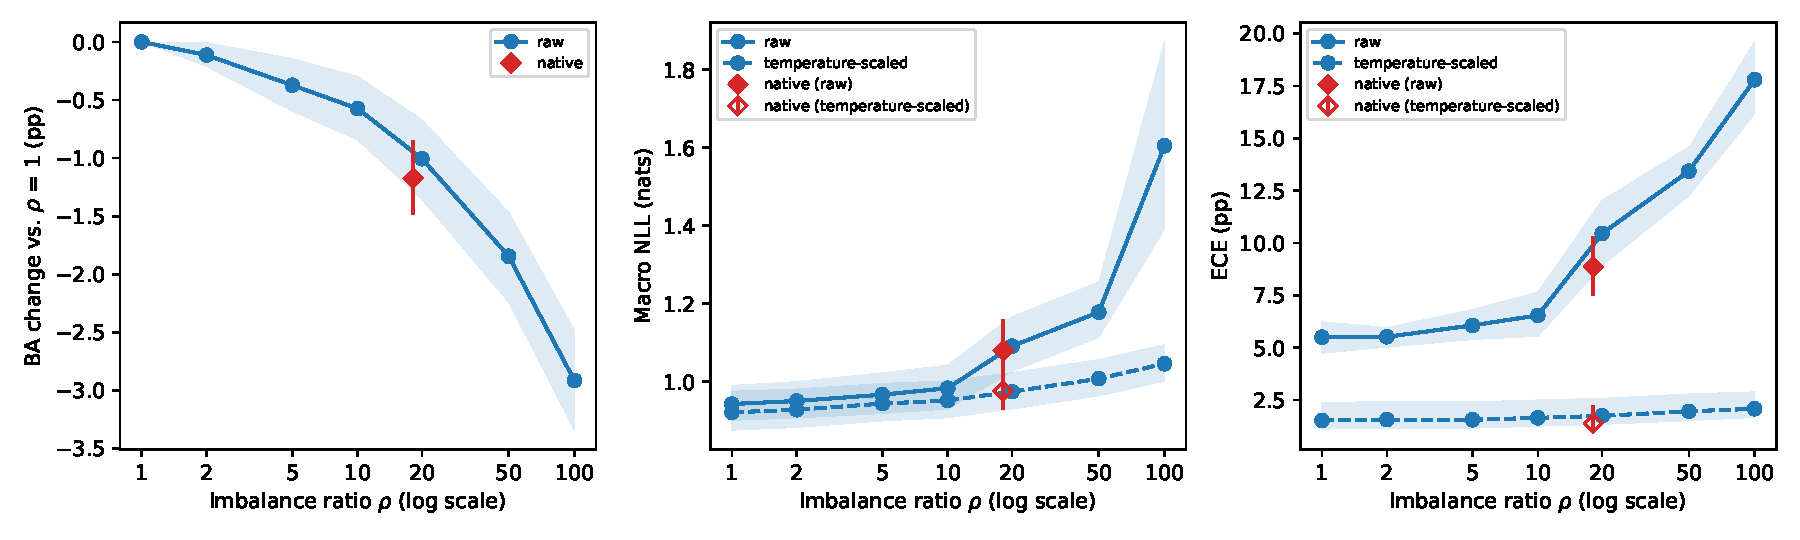
\includegraphics[width=\textwidth]{prevalence_curve.pdf}
\caption{Balanced accuracy degrades slowly and accelerates beyond $\rho=10$; raw calibration degrades much faster but recovers almost completely under temperature scaling. Blue lines connect the ratio arms at their realized ratio, with shaded paired 95\% bootstrap bands; the red diamonds mark the native allocation at its realized ratio of 18.1. Left: change in patient-macro balanced accuracy relative to the balanced arm. Middle and right: macro NLL and ECE, raw (solid, filled) and after validation temperature scaling (dashed, open).}
\label{fig:curve}
\end{figure}

\subsection{Where the damage lands}
\label{sec:rank-results}
The aggregate damage is the net result of a large redistribution of recall from the tail to the head (Table~\ref{tab:thirds}). In the balanced arm the three thirds of the class ranking reach the same recall, about 72 percent, as the random rank assignment implies. As $\rho$ grows, the head third gains up to 5.4 points and the tail third loses up to 11.8 points, while the body third loses 2.3 points at $\rho=100$. Because balanced accuracy weights all classes equally, the loss of the tail outweighs the gain of the head, and the balance between them worsens with $\rho$: at $\rho=10$ the tail loses 5.1 points against a head gain of 4.1, at $\rho=100$ it loses 11.8 against 5.4. The head gain saturates beyond $\rho=20$, whereas the tail loss keeps growing, which produces the acceleration of the curve.

\begin{table}[htbp]
\centering
\small
\renewcommand{\arraystretch}{1.15}
\begin{tabular}{@{}lrrrrrrr@{}}
\toprule
Third & r1 & r2 & r5 & r10 & r20 & r50 & r100 \\
\midrule
Head & 72.06 & 73.91 & 74.82 & 76.12 & 76.58 & 77.31 & 77.48 \\
Body & 72.19 & 72.15 & 71.74 & 71.48 & 71.00 & 70.51 & 69.87 \\
Tail & 71.92 & 69.77 & 68.49 & 66.85 & 65.57 & 62.81 & 60.08 \\
\bottomrule
\end{tabular}
\caption{Imbalance moves recall from the tail to the head, and the tail loses more than the head gains. Mean patient-macro recall in percent of the ten head, body, and tail classes of each draw, by their assigned rank, averaged over 30 fits. The native arm is omitted because its class order is not the random rank order that defines the thirds.}
\label{tab:thirds}
\end{table}

\subsection{Native allocation}
\label{sec:native-results}
The native class distribution of TCGA-UT costs 1.18 points against the balanced arm (0.85 to 1.48), just above the threshold. It lies on the ratio curve: interpolated at its realized ratio of 18.1, the curve predicts a damage of 0.93 points, and the native arm falls 0.25 points below it ($-0.57$ to 0.07), a difference whose interval contains zero. The native order ties prevalence to particular cancer types, whereas the ratio arms randomize that assignment, so this agreement indicates that the rare cancer types of TCGA-UT are not systematically harder or easier to learn from few patches than the average class. The native profile is also not exponential: its median class receives about 700 patches, whereas an exponential profile with the same extremes gives the median class about 400. The realized ratio alone nevertheless places it on the curve within the precision of this study.

\subsection{Probability quality}
\label{sec:calibration-results}
Raw probability quality degrades long before accuracy does, and most of the degradation is removed by a single temperature (Table~\ref{tab:curve}). Without scaling, the ECE stays near 5.5 points up to $\rho=2$ and rises to 10.45 points at $\rho=20$ and 17.80 points at $\rho=100$, an increase of 12.30 points (10.20 to 14.51). Macro NLL rises by 0.66 nats (0.46 to 0.91) at $\rho=100$. After temperature scaling, the increase at $\rho=100$ shrinks to 0.56 points of ECE (0.19 to 0.94) and 0.12 nats of NLL (0.11 to 0.14). Scaling therefore removes 95 percent of the ECE increase and 81 percent of the NLL increase. The scaled NLL increase that remains is resolved and follows the accuracy loss, since NLL also penalizes wrong predictions. The native arm shows the same pattern: its raw ECE exceeds that of the balanced arm by 3.36 points (1.50 to 5.31), and after scaling the difference is $-0.13$ points ($-0.38$ to 0.13).

The fitted temperatures show the direction of the miscalibration. The balanced arm is slightly underconfident, with a mean temperature of 0.84, and the temperature rises steadily with $\rho$ to 2.35 at $\rho=100$, where predictions must be softened by more than a factor of two. The selected regularization moves in the same direction: the balanced arm selects $\lambda=0.1$ in 28 of 30 fits, whereas $\rho=100$ selects $\lambda\leq10^{-3}$ in all 30 fits, and every selection lies inside the grid. Weaker regularization lets the logits grow, which produces overconfidence. The study does not separate this effect of model selection from the direct effect of the skewed class prior on confidence.

\section{Discussion}
\label{sec:discussion}
Of the three readings fixed in Section~\ref{sec:evaluation}, the results select the second: prevalence alone damages discrimination on TCGA-UT, but only from $\rho\approx20$, and by less than three points even at $\rho=100$. The third reading is not supported, because the native allocation lies on the curve. With patients and the total budget held fixed, a hundredfold imbalance leaves the tail classes with between one and two patches per patient, and the tail third of the classes still reaches 60 percent recall. Per doubling of the ratio, the loss is small below $\rho=10$ and grows to 0.7 points above it, which is where tail support per patient falls below eight patches.

The native TCGA-UT distribution, at a realized ratio of 18, is a modest imbalance for this dataset. Its damage of 1.18 points is small compared with the patient-count effects of this series: at 160 patches per class, going from five to twenty patients per class gains 9.41 points \citep{queisler2026centreError}. In a long-tailed TCGA-UT training set, the number of patients per class is therefore likely to matter more than the prevalence of the class, provided the rare classes still receive a few patches from each of their patients. The benchmark measured 1.33 to 1.79 points of severe-imbalance damage on TCGA-UT \citep{queisler2026benchmarkResults}, less than the 2.91 points at $\rho=100$ here. The designs differ in readout, reference allocation, patient pool, and budget, so the two magnitudes are not directly comparable; both place the damage of severe prevalence imbalance on TCGA-UT at a few points.

Calibration responds to prevalence much more strongly than discrimination, but in a form that one parameter repairs. The ECE triples at $\rho=100$ while accuracy loses four percent of its value, and validation temperature scaling on the natural validation distribution removes almost all of that ECE increase. This matches the benchmark's finding that most probability-quality benefits of prevalence weighting disappear after temperature scaling \citep{queisler2026benchmarkResults}. For TCGA-UT at fixed patient support, the calibration damage of imbalance is therefore mostly a uniform overconfidence that a post-hoc temperature removes, not a class-specific distortion. Prevalence-based corrections \citep{buda2018systematic} could still recover part of the tail recall, but they would have to beat a temperature-scaled baseline on probability quality to show value beyond it.

The next studies of the split-deprivation series vary patch count per class at fixed prevalence and patient count at fixed patch count, one factor at a time. Together with this curve, they will show which of the factors bundled in the benchmark carries its damage.

\section{Limitations}
\label{sec:limitations}
Each ratio moves the class prior and the tail support together, because the total budget is fixed; the study does not separate the effect of prevalence as such from the effect of the smaller per-patient patch count of the tail classes. A design at fixed tail support, with more patches for the head, would separate them. The twenty patients per class are the same in every arm, so the curve describes imbalance at adequate patient support; long-tailed datasets usually also have fewer patients in the rare classes, and that combination is left to the patient-shortage study.

The ratio grid ends at 100 and resolves the onset only to the grid spacing: the one-point damage is crossed between $\rho=10$ and $\rho=20$, and the damage at $\rho=20$ meets the threshold by its point estimate only. The native arm is a single allocation, so its agreement with the curve does not show that every class order behaves like a random one. Temperature scaling is fitted on a validation partition with the natural class distribution of TCGA-UT; under a different deployment prior, the calibration results may differ. All results are conditional on frozen Virchow2 features, multinomial logistic regression, TCGA-UT, and three overlapping splits.
